\documentclass[twoside,10pt]{article}

% Set Page Size And Margin Size
\usepackage[letterpaper,top=2cm,bottom=2cm,left=2.5cm,right=2.5cm,marginparwidth=1.75cm]{geometry}

% AMS Packages
\usepackage{amsmath,amsthm,amssymb,amsfonts}

% Formatting Packages
\usepackage{fancyhdr,biblatex,parskip,pgfplots}
\pgfplotsset{compat=1.18}
\usepackage{algorithm,algpseudocode}
\usepackage{inconsolata}
\usepackage{graphicx,subcaption,float}

% Externalize Figures 
\usepgfplotslibrary{external}
\tikzexternalize

% Set Up Header
\fancyhf{}
\fancyhead[LO,LE]{\nouppercase{\leftmark}}
\fancyhead[RO,RE]{\rightmark}
\fancyfoot[CO,CE]{\thepage}
\renewcommand{\headrulewidth}{0pt}
\pagestyle{fancy}

\fancypagestyle{lastpagefooter}{
    \fancyhf{} % Clear header and footer
    \renewcommand{\headrulewidth}{0pt} % Remove header rule
    \fancyfoot[C]{This document was produce in \LaTeX, the source code can be accesed at github.com/dyla-tr0n.}} % Footer content
\AtEndDocument{\thispagestyle{lastpagefooter}}

% Initalise Title
\title{P versus NP: Why it's difficult to say what's difficult.}
\author{Dylan Sneddon}
\date{}

% Import Bibliography File
\addbibresource{sample.bib}
% Begin Document
\begin{document}

\maketitle
\vspace{-0.75cm} % Compensate for the blank date.
\begin{abstract}
A brief introduction to computational complexity theory, the P versus NP problem and why it is so difficult to solve.
\end{abstract}

\section{Introduction}
How much money would you be willing to wager on a fact no one in world knows? £10, £100, £1000? How about £14.8 trillion? Sounds ridiculous, right? Well that gargantuan number represents how much the internet is worth\textsuperscript{\cite{cisco13}} and everyday we rely on an unproven result to uphold every single penny of it.

\begin{center} \centering The unproven result in question: the P versus NP problem.\end{center}

\section{The P vs NP Problem}
To make sense of that financial bombshell, we need to understand what the P versus NP problem is. Selected in the year 2000 by the Clay Maths Institute\textsuperscript{\cite{claymath}}, P versus NP is one of their seven Millennium Prize Problems - a group of unsolved mathematics problems deemed to be some of the hardest in contemporary mathematics. 

It is often written as: P$\stackrel{?}{=}$NP because the aim of the problem is to determine whether P is equal to NP. With no context, most mathematicians would laugh if you asked them if P$=$NP, as it could be solved like this:
\begin{align*}
    &P=NP\\
    &P-NP=0\\
    &P(1-N)=0\\
    &P=0,N=1
    &\text{The equation holds when P=0 or N=1 but not simultaneously.}
\end{align*}

On the other hand, if you approached a mathematician and asked to solve the millennium problem P$\stackrel{?}{=}$NP, they would laugh - but this time out of nervousness at the impossibility of the demand you've just placed upon them.

That begs the question; what are P and NP and why is it so difficult to tell if they're equal. P and NP both describe classes of mathematical and computational problems - a class is a collection of problems with a similar characteristic. P denotes the class of problems, which can be solved easily. Meanwhile, NP is the class of problems, which solutions can be verified easily. So P$\stackrel{?}{=}$NP aims to determine if the classes of P and NP are the same, that is to say: are all problems that are easy to verify also easy to solve?

A common example from cryptography is the factorisation of semi-prime numbers. A semi-prime number is a positive integer, with only two prime factors - when given a semi-prime number it is very challenging to find these two factors (due to the large amount of trial and error) so this problem is hard to solve. If given two factors we can easily multiply them together to see if they make the desired semi-prime so it is easy to verify solutions to this problem.

For example, if you were asked to find the two factors of 15347 a lot of trial and improvement would be needed to even come close to the answer. However, if you were told the factors were 103 and 149 you could easily verify this by showing 103x149=15347. As a result, we can say that the semi-prime factorisation problem is in the class NP but not in the class P.

It looks like we have just found an example which shows P$\neq$NP since the semi-prime factorisation was easy to verify solutions for but difficult to solve. However, we cannot say for certain that our current method of semi-prime factorisation is the most efficient, mathematicians may discover a very efficient method that would make this problem easy to solve so, right now we cannot say for certain whether such a method exists.

\subsection{Algorithms}
\textbf{Definitions:}
\begin{enumerate}
    \item \textbf{Algorithm -} A process or set of instructions, typically performed by a computer.
     \item \textbf{Execution -} Performing the instructions associated with an algorithm.
    \item \textbf{Input -} The data or information an algorithm receives and operates on.
    \item \textbf{Output -} The values produced by an algorithm, once it has been executed.
    \item \textbf{Termination -} When an algorithm is complete, and there are no instructions left to execute. 
\end{enumerate}

An algorithm can be used to describe anything, from performing simple calculations to challenging computational problems. They are vital to the PvsNP problem, as to calculate the difficulty of a problem we have to calculate the difficulty of the algorithm used to solve it. Figure 1 shows two different algorithms written in pseudocode, which is a format that cannot be processed by computers but represents the instructions one might perform.

% Pseudocode Algorithms
\begin{figure}[H]
\centering
\begin{minipage}[t]{0.4\textwidth}
\begin{algorithm}[H]
\caption{Odd Or Even Algorithm}
\begin{algorithmic}[1]
\State \texttt{let x be a positive integer}
\State \texttt{let y = x/2}
\State \texttt{if y is an integer:}
\State \texttt{output x is even}
\State \texttt{if y is not an integer:}
\State \texttt{output x is odd}
\end{algorithmic}
\end{algorithm}
\end{minipage}
\hspace{0.05\textwidth}
\begin{minipage}[t]{0.45\textwidth}
\begin{algorithm}[H]
\caption{Triangular Numbers Algorithm}
\begin{algorithmic}[1]
\State \texttt{let t = 0}
\State \texttt{let i = 1}
\State \texttt{let t = t+i}
\State \texttt{output t}
\State \texttt{increment i by one}
\State \texttt{return to step 3}
\end{algorithmic}
\end{algorithm}
\end{minipage}
\caption{Two Pseudocode Algorithms}
\label{fig:algorithmintro}
\end{figure}

Figure 1 demonstrates that an algorithm is just a series of processes that can be performed in order. Algorithm 1 determines the parity of a positive integer $x$. Algorithm 2 generates the sequence of triangular numbers. There is one key difference between the two algorithms, that is Algorithm 1 is terminating whilst Algorithm 2 is non-terminating. Algorithm 1 terminates once it has outputted whether $x$ is odd or even, whilst Algorithm 2 returns to step 3 on the final line thus never reaching the end. We only consider terminating algorithms because a non-terminating algorithm runs forever. This means they are neither easy nor difficult to perform completely, they're impossible to perform completely.

\subsection{Sets}
Now we understand what an algorithm is, but recall the P versus NP problem; we want to determine if the P and NP problem classes are the same. Classes are rigid mathematical objects that are hard to compare and operate on, fortunately they are analogous to another mathematical object known as a set. We will consider the P and NP classes as two sets called P and NP. Sets are some of the most basic structures in mathematics, and hence there is heavy debate about what constitutes a set. For our purposes, a set is a collection of objects those objects are called the elements of the set. 

Sets are denoted by curly braces with commas separating the elements. {$\{0,1,2,3\}$} is the set of the first four positive integers - the order of the elements of a set does not matter and sets cannot contain duplicate elements. That is to say, {$\{1,2\}$}, {$\{2,1\}$} and {$\{1,1,2\}$} represent the same set. To say $x$ is an element of a set $S$, we write it as $x\in S$. We can also specify a property of a set $\{x\in S:x\leq5\}$, this means the set of all the elements in the set $S$ that are less than or equal to 5.

As well as defining sets, set theory also allows us to describe how sets are related. We say that a set $X$ is a subset of a set $Y$ is all of the elements of $X$ are elements of $Y$ - conversely $Y$ would be a superset of $X$. We show this by $X\subseteq Y$, where $\subseteq$ means 'is a subset of'.

Finally, sets have a properly known as cardinality, which describes their size. The cardinality of a finite set is just the number of elements in the set. We can write the cardinality of a set $S$ as $\lvert S\rvert$. If $S=\{4,6,8\}$ then $\lvert S\rvert=3$ because $S$ has three elements.

You have probably seen some sets in mathematics, some of the most common examples include:
\begin{align*}
    \O &= \{\}&\text{The Empty Set}\\
    \mathbb{N} &= \{0,1,2,3,...\}&\text{The Natural Numbers}\\
    \mathbb{Z} &= \{0,\pm 1,\pm 2,\pm 3,...\}&\text{The Integers}\\
    \mathbb{Q} &= \{\dfrac{a}{b}:a,b\in\mathbb{Z},b\neq0\}&\text{The Rational Numbers}\\
    \mathbb{R} &= \{x:-\infty<x<\infty\}&\text{The Real Numbers}
\end{align*}
Sets are much more versatile than this, in most branches of mathematics sets follow a set of rules called the ZF axioms. As a result, most mathematical objects can be placed inside of a set.
\[\text{A Set of Sets: }\{\text{\O},\{-1\},\{1\}\{-1,1\}\}\quad\text{(The set of all subsets of $\{-1,1\}$, called the power set of $\{-1,1\}$.)}\]
\[\text{A Set of Vectors: }\{\begin{pmatrix}a_{1}\\\vdots\\a_{n}\end{pmatrix}:a_{i}\not\in\mathbb{N}\}\quad\text{(The set of all $n$-dimensional vectors with non-natural components.)}\]

Clearly, if sets can contain other sets and vectors we are able to create a set with other mathematical objects. We could therefore create two sets and fill them with algorithms; one set for the algorithms that are easy to perform. And one set for the algorithms that are easy to verify.
\begin{align}
    \text{P} &= \{\text{algorithms}:\text{algorithm is easy to perform}\}\\
    \text{NP} &= \{\text{algorithms}:\text{algorithm is easy to verify}\}
\end{align}
These are naive definitions of a set, and we will refine them once we decide the criteria for an algorithm being easy or difficult. Nevertheless, we've obtained the mathematical tools to make such a classification.

Right now we can clearly say that P$\subseteq$NP as all problems with algorithms that are easy to perform can have solutions verified easily as well. However, as shown earlier with semi-prime factorisation we do not know if NP$\subseteq$P, as some easy to verify problems may always be hard to solve. 

If it turns out than in addition to P being a subset of NP that NP is also a subset of P then P must equal NP. This is a process known as double inclusion. If P is a subset of NP and NP is a subset of P then P must be the same set as NP. This is one potential and powerful method that could be used to solve the P vs NP problem.

\section{Complexity Theory}
P versus NP hinges on the idea of certain algorithms begin easy to perform and others being difficult to perform. Despite being a pretty intuitive concept, currently we don't have a method of determining the difficulty of an algorithm - that's where computational complexity theory comes in. Now, I can hear you saying:

``This is supposed to be a maths essay but you have just use the word computational. You've tricked me into reading about a different subject, how dare you!''

Fear not! Complexity theory, like most of computer science, is grounded in mathematics. This means that we're going to start from the very beginning and discover complexity theory from its fundamental building blocks. To do this, we will take a top-down approach, starting with the big questions and assumptions and filling in the small details later. Clearly, the biggest question is, what does complexity theory aim to achieve? 

Complexity Theory, in the simplest form, exists to categorise algorithms into categories: easy to execute or difficult to execute. So perhaps the first building block would be to decide what easy and difficult mean.

\subsection{Difficulty}
\textbf{Definitions:}
\begin{enumerate}
    \item \textbf{Time Complexity -} The length of time it takes for the algorithm to terminate, with respect to the size of the data input into it.
\end{enumerate}
We know what algorithms are, and we have the tools to categorise them. It is time to finally decide how to say which algorithms are difficult. If you're particularly perceptive you may have realised that we will be considering time complexity for complexity theory.

There are many misconceptions about what time complexity actually measures. Time complexity measures how the time taken for an algorithm to terminate grows as the size of input into it increases. The easiest way to imagine this is a graph with input size on the $x$-axis and termination time on the $y$-axis.
\begin{figure}[h]
\centering
\begin{subfigure}{0.45\textwidth}
\centering
\begin{tikzpicture}
\begin{axis}[
    xlabel={Input Size$\rightarrow$},
    ylabel={$\uparrow$Termination Time},
    axis lines=middle,
    xmin=0, xmax=5,
    ymin=0, ymax=3,
    xtick={0,1,2,3,4,5},
    ytick={0,1,2,3},
    xticklabels={},
    yticklabels={},
    grid=none,
    ticks=none,
    tick style={draw=none},
    samples=10,
]
\addplot[domain=0:5, samples=100, black] {sqrt(x)};
\end{axis}
\end{tikzpicture}
\caption{Termination Time is Increasing Slowly, as Input Size Increases. This Represents an Easy Algorithm.}
\label{fig:radicalgraph}
\end{subfigure}
\hspace{0.5cm}
\begin{subfigure}{0.45\textwidth}
\centering
\begin{tikzpicture}
\begin{axis}[
    xlabel={Input Size$\rightarrow$},
    ylabel={$\uparrow$Terminaton Time},
    axis lines=middle,
    xmin=0, xmax=5,
    ymin=0, ymax=32,
    xtick={0,1,2,3,4,5},
    ytick={0,2,4,8,16,32},
    xticklabels={},
    yticklabels={},
    grid=none,
    ticks=none,
    tick style={draw=none},
    samples=2,
]
\addplot[domain=0:5, samples=100, black] {2^x};
\end{axis}
\end{tikzpicture}
\caption{Termination Time is Increasing Quickly, as Input Size Increases. This Represents a Difficult Algorithm.}
\label{fig:exponentialgraph}
\end{subfigure}
\caption{Termination Time Shown As Two Different Functions of Input Size}
\label{fig:comparison}
\end{figure}

As you can see from figure 2, as the size of the data input into an algorithm increases, time also increased. However as shown in the left graph it can increase at a slow rate - this is the property of an easy algorithm. Meanwhile, the graph on the right shows that termination time can increase quickly when compared to input size, a property of a difficult algorithm.

Notice there are no numbers on either axis. That is because in complexity theory we are not interested in individual values of input size or time - just how time changes with respect to input size. Imagine plotting a graph of input size against termination time and then putting a sticker over the axes as to obscure the numbers - that is what we do in complexity theory.

Why do we obscure the axes and no consider individual values of time? In a modern computer science context it wouldn't be sensible to consider values of time, as the length of time it takes an algorithm to terminate depends on the hardware that's running it but no matter how powerful the hardware termination time grows at the same rate. See figure 3 for an example.

\begin{figure}[H]
    \centering
    \includegraphics[width=0.5\linewidth]{HardwareTime.png}
    \caption{The Supercomputer Solves the Sudoku Faster than the Potato}
    (But as the Sudoku Gets Bigger, Termination Time Will Increase at the Same Rate for Both of Them.)
    \label{fig:hardware}
\end{figure}


\subsection{Functions}
Since the difficulty of an algorithm can be determined by the shape of the graph of input size against time we require time as function of input size for each algorithm in order to determine its difficulty.

This type of function is known as a time complexity function, a function $t(n)$ that takes input size $n$ and maps it to time $t$. Recall, we don't consider individual values of time or input size so once the graph is sketched these values must be omitted from the axis. Therefore, we require a function that can map input lengths to termination times:
\[t(n) \text{ is a function that takes algorithmic input length $n$ such that }t:\mathbb{N}\rightarrow\mathbb{R}^+.\]

The P versus NP problem aims to find whether all problems that are easy to verify are easy to solve. So we can start generating time complexity functions by taking an algorithm we know is easy to verify and seeing if it is easy to solve.

Our algorithm will take a list of numbers length $n$ and find if the number 7 is in the list; this will be called the 7 finding algorithm. For the sake of simplicity we will make the following assumptions:
\begin{enumerate}
    \item Assume it takes $k$ seconds to check if each number is 7 or not. Where $k$ is a positive constant.
    \item Assume each list searched by the algorithm contains has exactly one 7.
\end{enumerate}

To find the running time of this algorithm we need to find the average number of checks the algorithm will perform, based on the number of length of the list. This can  also be known as the expected value of checks. Let $X$ represent the number of checks until 7 is found. In order to estimate the value of $X$ we can find the expected value of $X$ for each value of $n$. The equation for the expected value of this probability distribution is given by:
\[E_{n}(X)=\sum_{i=1}^nikP(X=i)\]
Where $E_{n}(X)$ is the expected number of checks for a list length $n$, $k$ is the number of seconds per check and $P(X=i)$ is the probability $i$ checks are needed.

This means the expected value for a given input length $n$ is the sum of each number of possible checks multiplied by the probability of that happening multilpied by the time taken per check. For example in a list of 4 numbers each has a $\frac{1}{4}$ chance of being the number 7.
\begin{figure}[h]
\centering
\begin{center}
\begin{tabular}{ c c c c }
 5 & 3 & 7 & 2\\
 $\frac{1}{4}$ & $\frac{1}{4}$ & $\frac{1}{4}$ & $\frac{1}{4}$
\end{tabular}
\end{center}
\caption{Each Number in the List has a 1/4 Chance of Being the Number 7.}
 \label{fig:fourlist}
\end{figure}

As you can see, if seven is in a random position in that list is a $25\%$ we find it on each attempt. This means the expected value is can be found with:
\begin{equation*}
    E_{4}(X)=k\times\dfrac{1}{4}+2k\times\dfrac{1}{4}+3k\times\dfrac{1}{4}+4k\times\dfrac{1}{4}=\dfrac{k}{4}\left(1+2+3+4\right)
\end{equation*}
More generally for a list of $n$ numbers the chance of finding 7 on any attempt is $\dfrac{1}{n}$. Consequently, the general form for the expected value is given by:
\[E_{n}(X)=\dfrac{k}{n}\left(\sum_{i=1}^ni\right)\]
That summation is the sum of the first $n$ natural numbers, it turns out that we can also express that sum as $\frac{n(n+1)}{2}$. Therefore we can express the termination time of the 7 finding algorithm as a function of input size.
\begin{align*}
    E_{n}(X)&=\dfrac{k}{n}\left(\sum_{i=1}^ni\right)\\
    &=\dfrac{k}{n}\left(\frac{n(n+1)}{2}\right)\\
    &=\frac{k(n+1)}{2}\\
    &=\dfrac{k}{2}n+\dfrac{k}{2}
\end{align*}
Therefore the time complexity function for the 7 finding algorithm is $\dfrac{k}{2}n+\dfrac{k}{2}$. Remember that $k$ is just the amount of time per check, and is therefore just an arbitrary positive constant. We will consider the graph of this function in order to determine whether the algorithm is easy or difficult to execute. 

\begin{figure}[h]
    \centering
    \begin{tikzpicture}
  \begin{axis}[
    axis lines=middle,
    xlabel={Input Size($n$)},
    ylabel={Time Taken},
    ymin=0,ymax=2,  
    xtick={0,1,2,3},
    xticklabels={0,1,2,3},
    domain=0:3,
    samples=5,
    ]
    \addplot[black] {0.5*x+1/2};
  \end{axis}
\end{tikzpicture}
    \caption{The Time Complexity Function of the Seven Finding Algorithm}
    \label{fig:lineargraph}
\end{figure}

\begin{figure}[H]
Figure 5 illustrates that the time complexity function is linear, meaning the execution time grows at a constant rate with respect to input size, this is slow enough growth to categorise our algorithm as easy. When considering time complexity, we only look at the leading term of the time complexity function ignoring coefficients to decide the difficulty since this is the term that determines the shape of the function - see Figure 6.

\begin{tikzpicture}
  \begin{axis}[
    axis lines=middle,
    xlabel={$x$},
    ylabel={$y$},
    ymin=0,ymax=10,  
    xtick={-3,-2,-1,0,1,2,3},
    xticklabels={-3,-2,-1,0,1,2,3},
    domain=-4:4,
    samples=50,
    ]
    length=6cm
    \addplot[black] {x^2-4*x+4};
    \addlegendentry{\(x^2 - 4x + 4\)}
  \end{axis}
\end{tikzpicture}
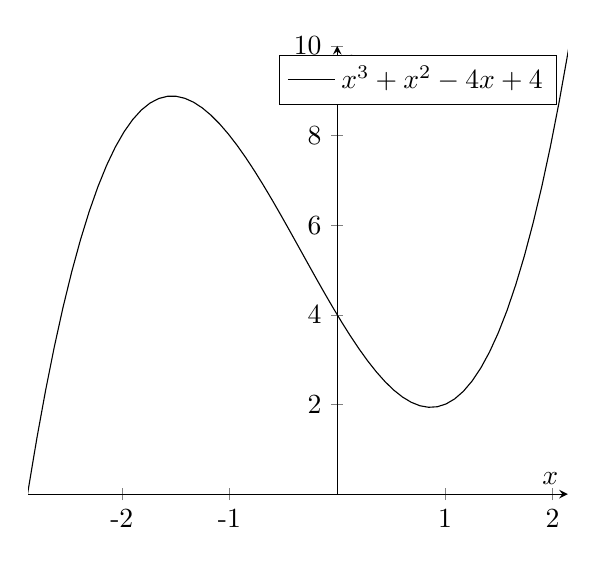
\begin{tikzpicture}
  \begin{axis}[
    axis lines=middle,
    xlabel={$x$},
    ylabel={$y$},
    ymin=0,ymax=10,  
    xtick={-3,-2,-1,0,1,2,3},
    xticklabels={-3,-2,-1,0,1,2,3},
    domain=-4:4,
    samples=100,
    ]
    length=6cm
    \addplot[black] {x^3+x^2-4*x+4};
    \addlegendentry{\(x^3 + x^2 - 4x + 4\)}
  \end{axis}
\end{tikzpicture}
\caption{Both Functions Share The Same Final Three Terms, But The Leading Term Determines The Shape}
\label{fig:shapegraph}
\end{figure}
\vspace{-20pt}
This method has produced the time complexity function for one algorithm, clearly this is not very efficient and we need a general way of generating time complexity functions to even come close to solving P versus NP. 
\vspace{-20pt}
\subsection{Big O Notation}
We are approaching mastery of complexity theory. We know what algorithms are, we have found how to use sets to group them, and we have created functions to determine the time complexity of an algorithm. All that is left to do now is to decide, which algorithms are members of the set P and which algorithms are members of the set NP.

This is where we will use Big O Notation, a way of quickly describing the time complexity of an algorithm with respect to input size. Big O Notation tells us the leading term of an algorithm's time complexity function, allowing us to easily infer the difficulty.

Big O Notation, is easy to understand. If an algorithm's time complexity function is described by $3n^2+5n+2$ then the Big O Notation for the algorithm is $O(n^2)$. If an algorithms time complexity function is $\log{n}+n!$ then its Big O Notation is $O(n!)$.Some further examples in order of time complexity include:
\begin{itemize}
    \item Constant Time - $O(1)$
    \item Logarithmic Time - $O(\log{n})$
    \item Polynomial Time - $O(n^k),k\in\mathbb{N}$
    \item Exponential Time - $O(2^n)$
    \item Factorial Time - $O(n!)$
\end{itemize}

Each of the above examples represents a set of algorithms, $O(2^n)$ represents the set of algorithms that terminate in exponential time. As a result, we can say that an algorithm $A$ is part of the exponential time set using the notation $A\in O(2^n)$. Figure 8 illustrates how efficient each different time complexity is:
\begin{figure}[H]
\centering
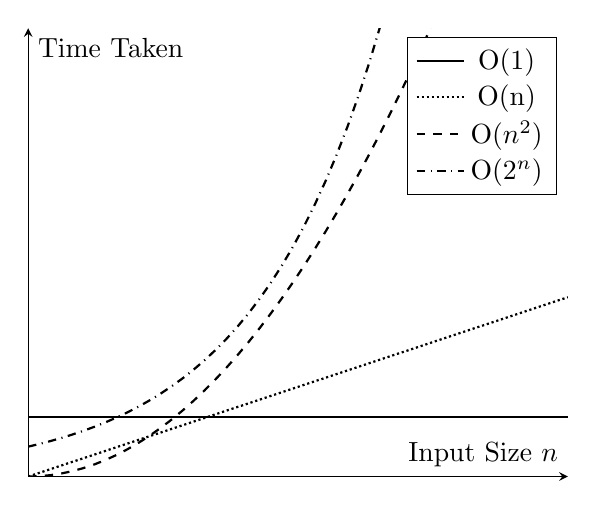
\begin{tikzpicture}
  \begin{axis}[
    axis lines=middle,
    xlabel={Input Size $n$},
    ylabel={Time Taken},
    ymin=0,ymax=15,  
    ticks=none,
    tick style={draw=none},
    domain=0:6,
    samples=50,
    ]
    \addplot[thick] {2};
    \addplot[densely dotted][thick] {x};
    \addplot[dashed][thick] {0.75*x^2};
    \addplot[dash dot][thick] {2^x};
    \legend{O(1),O(n),O($n^2$),O($2^n$)}
  \end{axis}
\end{tikzpicture}
\caption{Examples Of How Big O Notation Represents Time Complexity}
\label{fig:ograph}
\end{figure}
So, what is the threshold for a problem being difficult? Computer scientists have decided that any algorithm with a time complexity of more than $O(n^k)$ is considered difficult. This means that every polynomial and logarithmic time algorithm are considered easy and conversely exponential time algorithms are always hard.
\begin{proof} - Proof that all exponential time algorithms are difficult.

Consider two arbitrary functions $f(x)$ and $g(x)$. If the leading term of $f(x)$ grows faster than the leading term of $g(x)$ then as $x\rightarrow\infty$, $\frac{f(x)}{g(x)}\rightarrow\infty$. 

Therefore, if an algorithm is more time complex than $O(n^k)$ - and hence difficult - as $n\rightarrow\infty$, $\frac{f(n)}{n^k}\rightarrow\infty$ where $f(n)$ is the leading term of some difficult algorithm's time complexity function.

In order to prove all exponential time algorithms are difficult, we want to show they grow faster than all polynomial time algorithms. Hence we want to show that:
\[\lim_{n\to\infty}\dfrac{2^n}{n^k}=\infty\quad\forall k\in\mathbb{N}\]

Substituting into this limit gives an indeterminate form of $\frac{\infty}{\infty}$. Fortunately, we can use L'Hôpital's rule which states:
\[\lim_{x\to c}\dfrac{f(x)}{g(x)}=\lim_{x\to c}\dfrac{f'(x)}{g'(x)}\]

Initially, this will continue to give indeterminate forms of $\frac{\infty}{\infty}$ but we can reapply L'Hôpital's rule $k$ times until we reach the $k$th derivative of $2^n$ and $n^k$. It turns out the $k$th derivative of $2^n$ is $2^n\ln^k{(2)}$ and the $k$th derivative of $n^k$ is $k!$. Using these derivatives we can finally evaluate the limit.
\[\lim_{n\to\infty}\dfrac{2^n}{n^k}=\lim_{n\to\infty}\dfrac{\dfrac{d^k}{dn^k}2^n}{\dfrac{d^k}{dn^k}n^k}=\lim_{n\to\infty}\dfrac{2^n\ln^k{(2)}}{k!}=\dfrac{\infty}{k!}=\infty\]

Because $k!$ is jut a constant we know that $\frac{\infty}{k!}=\infty$.  We have now shown the limit as $n$ tends to $\infty$ of the ratio is $\infty$ and therefore exponential algorithms are more time complex than all polynomial algorithms and therefore by definition are difficult to execute.
\end{proof}

Returning to the seven finding algorithm, its time complexity function was $\dfrac{k}{2}n+\dfrac{k}{2}$ and because $k$ is just a constant the leading term is $\dfrac{k}{2}n$ and the algorithm's time complexity is $O(n)$. Clearly this is an example of polynomial time so this is an algorithm describes a probem that is easy to solve and easy to verify.

What if we extend the 7 finding algorithm from earlier? Now it is going to check every pair of numbers in the list and see if they add together to give 7. This algorithm is still easy to verify, we check both numbers are in the lit an then add them. It turns out the time complexity for executing the algorithm is $O(n^2)$, another polynomial time complexity so this algorithm describes a problem that is easy to solve and verify.

Extending the algorithm further, if we make it check every triple of numbers in the list to see if any sum to 7 this has a time complexity of $O(n^3)$, whilst still being easy to verify and solve.

However, what if we asked the algorithm to find all combinations of numbers in a list that add to seven? If we imagine the list as a set of numbers and call that set $S$, we need to find the sum of the elements of every subset of that list. Recall that the set of all subsets of $S$ is known as the power set of $S$ which is denoted by $\mathcal{P}(S)$. If we can find a formula for the cardinality of the power set this will give us the time complexity function for the algorithm. It turns out that the cardinality of $\mathcal{P}(S)$ is equal to $2^n$ where $n=\lvert S\rvert$ - we can show this by induction:
\begin{proof} 
    We are going to show that if $\lvert S\rvert=n$ this implies that $\lvert\mathcal{P}(S)\rvert=2^n$.

\textbf{Base Case:} $n=0$

When $n=\lvert S\rvert=0$ then $S$ must be equal to the empty set $(S=\O)$. 

$\mathcal{P}(\O)$=$\{\O\}$ (The empty set only has one subset, itself.)

 $\lvert\mathcal{P}(\O)\rvert=1=2^0$

So the statement holds for the base case of $n=0$.

\textbf{Inductive Hypothesis:} Assume the statement holds for some $n=k,k\in\mathbb{N}.$

$\lvert S\rvert=k\implies\lvert\mathcal{P}(S)\rvert=2^k$

\textbf{Inductive Step:} Assuming the statement holds form some $n=k$, show this implies that it holds for $n=k+1$.

We want to show that: $\lvert S\rvert=k+1\implies\lvert\mathcal{P}(S)\rvert=2^{k+1}$

Let $\lvert S\rvert=k+1$. Let $z$ be some arbitrary element of $S$ such that $z\in S$. Let $S_{2}$ be the set $S$ with the element $z$ removed from it.

$\lvert S_{2}\rvert$=k and from the inductive hypothesis $\lvert\mathcal{P}(S_{2})\rvert=2^k$. Now consider $\mathcal{P}(S)$, this is just the set containing $\mathcal{P}(S_{2})$ and all subsets of $S_{2}$ with $z$ added into them. Since $\lvert\mathcal{P}(S_{2})\rvert=2^k$ adding $z$ to every subset of $S_{2}$ will just make $2^k$ more subsets. Therefore, $\lvert\mathcal{P}(S)\rvert=2^k+2^k=2\times 2^k=2^{k+1}$.

Hence, given that the statement hols for $n=k$ it holds for $n=k+1$ meaning by induction it holds for all natural numbers $n$. Therefore we have shown, $\lvert S\rvert=n\implies\lvert\mathcal{P}(S)\rvert=2^n$.
\end{proof}

Since the power set has $2^n$ elements, the time complexity of this version of the seven finder algorithm is $O(2^n)$, this is exponential time which grows faster than polynomial time and hence this is an algorithm that is easy to verify but difficult to solve.

Once again, this is where P vs NP becomes a challenge we cannot use this as a concrete example that P$\neq$NP since there may be a more efficient way to check all subsets that exists in polynomial time. And in the case such an example doesn't exist we would need to show that it is impossible to do that algorithm in a way that is any more efficient, which is a very tricky task.

\section{Why it's difficult to say what's difficult.}

it would be worthwhile reminding ourselves what the P versus NP problem asks. It asks if P, the set for which problems that are easy to solve, is equal to NP, the set of problems for which solutions can be easily verified. Obviously, if the two sets P and NP are equal they have the same elements. But what are the elements of each set? Using the set builder notation previously described we can define the sets as:
\begin{align*}
    \text{P} &= \{\text{algorithms}:\text{algorithm is easy to perform}\}\\
    \text{NP} &= \{\text{algorithms}:\text{algorithm is easy to verify}\}
\end{align*}

These are not a mathematically rigorous definition of a set, but using our knowledge of Big O Notation we can create some stricter rules to define which algorithms go in the set P. P stands for polynomial time, so this is the set of algorithms that can be executed in polynomial time or even more efficiently. NP stands for non-deterministic polynomial time, this is th set of algorithms tat can have solutions verifid in polynomial time. If we let the leading term of an algorithm's time complexity function be represented by $t(n)$ we can say:
\begin{align*}
    \text{P} &= \{\text{algorithms}:\exists k\in\mathbb{N} \text{ s.t.}\lim_{n\to\infty}\dfrac{n^k}{t(n)}=\infty\}
\end{align*}
What this says, is that P is the set of algorithms where there exists a value of $k$ such that $n^k$ grows faster than the algorithm' leading term. If such a value of $k$ doesn't exist then the algorithm is more time complex than every polynomial function making it difficult to execute.

So given that we can produce mathematically rigorous definitions of the set P, why is the problem so challenging? The difficulty lies in the absolute nature of P versus NP. To show that P$=$NP we would have to show that every single possible algorithm that is easy to verify can be solved easily. Conversely, to show that P$\neq$NP we would need to find a problem that is easy to verify and demonstrate that no matter what, it could not be solved in polynomial time.

Delving deeper into both outcomes, lets say we thought that P does indeed equal NP. What methods could we use to try and show this? We discussed double inclusion earlier, since we know P is a subset of NP, if we can show that NP is a subset of P they must be equal. The issue here is that we would need to come up with a property all algorithms in NP have meaning they must belong to P, and that is hard to find. There is also a class of problems called NP-hard, these are the hardest problems to execute in NP. If a polynomial time solution could be found for one, this would imply that all problems in NP can be solved in polynomial time. Finding a solution here is unlikely though as NP-hard problems involve discrete mathematics problems such as the Bin Packing and the Hamiltonian Cycle problem, which involved large amounts of permutations and trial and error that'll be difficult to overcome.

Advocating for the other side, if we wanted to show that P doesn't equal NP we only need to focus on one problem in NP instead of the entire set. Despite the fact that makes this route sound easier due to the smaller scope the path is beset with challenges here to. Using a method such as proof by contradiction, we would need to show that there exists an algorithm such that the most efficient way it could be executed was more time complex than polynomial time. In a world where everything is always improving and getting faster it will inevitably be difficult to show the lower bound of efficiency for an algorithm is not polynomial.

This is why it is difficult to say what is difficult, there is an infinite amount of algorithms in the world, an a seemingly infinite number of outcomes for each. It is easy for us to say which algorithms are definitely in P - it is easy to say what is easy. Sadly, it appears there will always be ambiguity about which algorithms are in NP but not P, making it truly difficult to say what is difficult.

\section{Conclusion}
No matter which way you look at it, P versus NP looks as if it will continue to evade mathematicians for decades. Most people in the field believe that P is not equal to NP and there are in fact some problems in NP that cannot be solved in polynomial time. 

Some people view this as a baseless claim, as there is little evidence to support this other than `what feels right'. Other people think the believe P isn't equal to NP is nervous optimism. Remember that £14.8 trillion, every day that P is not equal to NP all that money invested into the infrastructure of the Internet stay safe. Encryption algorithms all over the internet rely on being easy to verify to insiders with passwords called keys, but difficult to solve to those on the outside without the keys to decrypt the information. If researches are able to show that P equals NP suddenly most encryption algorithms on the internet fails as outsiders can easily break into them leaving everyone's sensitive data that travels across the internet free for public viewing.

Maybe we should stop researching P versus NP, in case the out come is that they are equal. Is it worth while to forfeit one piece of knowledge to protect the rest? Is it feasible to halt the advance of mathematics, just in case something goes wrong? Is it right to attach such large sums of money to a very narrow outcome? Whatever you think the answers to these questions are, there is no denying they could be difficult to find. But does that mean an algorithm finding the solution to P versus NP has to be considered in the problem itself? There's only one mathematical to describe that situation and it also begins with P. The word - paradox.

\printbibliography
\end{document}